% Poster for MACS 30200 — Judy Chen (REVISED v12)
% Standard 3-column layout
% 36" x 48" landscape = 91.44cm x 121.92cm

\documentclass[final]{beamer}

% ====================
% Packages
% ====================

\usepackage[T1]{fontenc}
\usepackage{lmodern}
\usepackage[size=custom,width=121.92,height=91.44,scale=1.0]{beamerposter}
\usetheme{gemini}
\usecolortheme{uchicago}
\usepackage{graphicx}
\usepackage{booktabs}
\usepackage[patch=none]{microtype}
\usepackage{tikz}
\usepackage{anyfontsize}

% Increase caption font size for poster readability
\setbeamerfont{caption}{size=\small}

\pdfstringdefDisableCommands{%
\def\translate#1{#1}%
}

% ====================
% Lengths
% ====================

\newlength{\sepwidth}
\newlength{\colwidth}
\setlength{\sepwidth}{0.025\paperwidth}
\setlength{\colwidth}{0.3\paperwidth}

\newcommand{\separatorcolumn}{\begin{column}{\sepwidth}\end{column}}

% ====================
% Title
% ====================

\title{Predicting Attention from the Surface: \\ Movie-Calibrated fNIRS as a Proxy for Whole-Brain fMRI}

\author{Judy Chen}

\institute[shortinst]{MACS 30200: Computational Research Design \\ University of Chicago \quad $\cdot$ \quad Advisor: Yuan Chang Leong}

% ====================
% Footer
% ====================

\footercontent{
  \href{https://github.com/judycchen/30200_proposal}{github.com/judycchen/30200\_proposal} \hfill
  MACS 30200 Poster Session --- Spring 2026 \hfill
  \href{mailto:judycchen@uchicago.edu}{judycchen@uchicago.edu}}

% ====================
% Body
% ====================

\begin{document}
\addtobeamertemplate{headline}{}
{
    \begin{tikzpicture}[remember picture,overlay]
      \node [anchor=north west, inner sep=3cm] at ([xshift=0.0cm,yshift=1.0cm]current page.north west)
      {
\includegraphics[height=5.0cm]{logos/uc-logo-white.eps}};
    \end{tikzpicture}
}

\begin{frame}[t]
\begin{columns}[t]
\separatorcolumn

% ====================
% COLUMN 1: Motivation, RQ, Study Design, start of Results (ISFC)
% ====================

\begin{column}{\colwidth}

  \begin{block}{Motivation}

    Individual differences in attention predict academic achievement, mental health outcomes, and occupational performance --- but the best tool for studying their neural basis, fMRI, is expensive, immobile, and concentrated in well-funded institutions. This excludes the populations most affected by attentional difficulties from the science that studies them.

    \textbf{Can a brief, portable brain recording approximate whole-brain neural measurement without a scanner?}

    Functional near-infrared spectroscopy (fNIRS) is lightweight and deployable in schools, clinics, and community settings, but it only measures cortical surface activity. Building on Gao et al.\ (2025), who showed fNIRS-to-fMRI prediction is possible within a single paradigm, this project tests whether such mappings generalize to structured cognitive tasks --- enabling field-deployable neurocognitive assessment of attention without scanner access.

  \end{block}

  \begin{alertblock}{Research Question}

    Can an fNIRS-to-fMRI mapping trained on movie-watching \textbf{generalize to cognitive tasks}, such that the predicted whole-brain patterns \textbf{correlate with individual differences in attention}?

    \medskip

    \textbf{Sub-questions:}
    \begin{enumerate}
      \item Which brain regions maintain stable fNIRS$\rightarrow$fMRI mapping across paradigms, and do these include the attention networks needed for individual-differences prediction?
      \item Can the model detect load-dependent differences (1-back vs.\ 2-back) that correlate with behavioral measures of attentional stability?
    \end{enumerate}

  \end{alertblock}

  \begin{block}{Study Design}

    fNIRS and fMRI data come from \textbf{different participant groups} who watched the same Hitchcock film clip (\textit{North by Northwest}, $\sim$15 min, 886 shared timepoints at TR $\approx$ 1\,s). The shared temporal structure allows a model to learn a mapping between modalities without simultaneous recording.

    \begin{figure}
      \centering
      
\includegraphics[width=0.98\textwidth]{figures/pipeline_diagram.pdf}
    \end{figure}

  \end{block}

  \begin{block}{Preliminary Results: Movie-Watching Training Phase}

    \heading{Large-scale connectivity structure preserved ($r = 0.552$, $p = 0.001$)}

    \begin{figure}
      \centering
      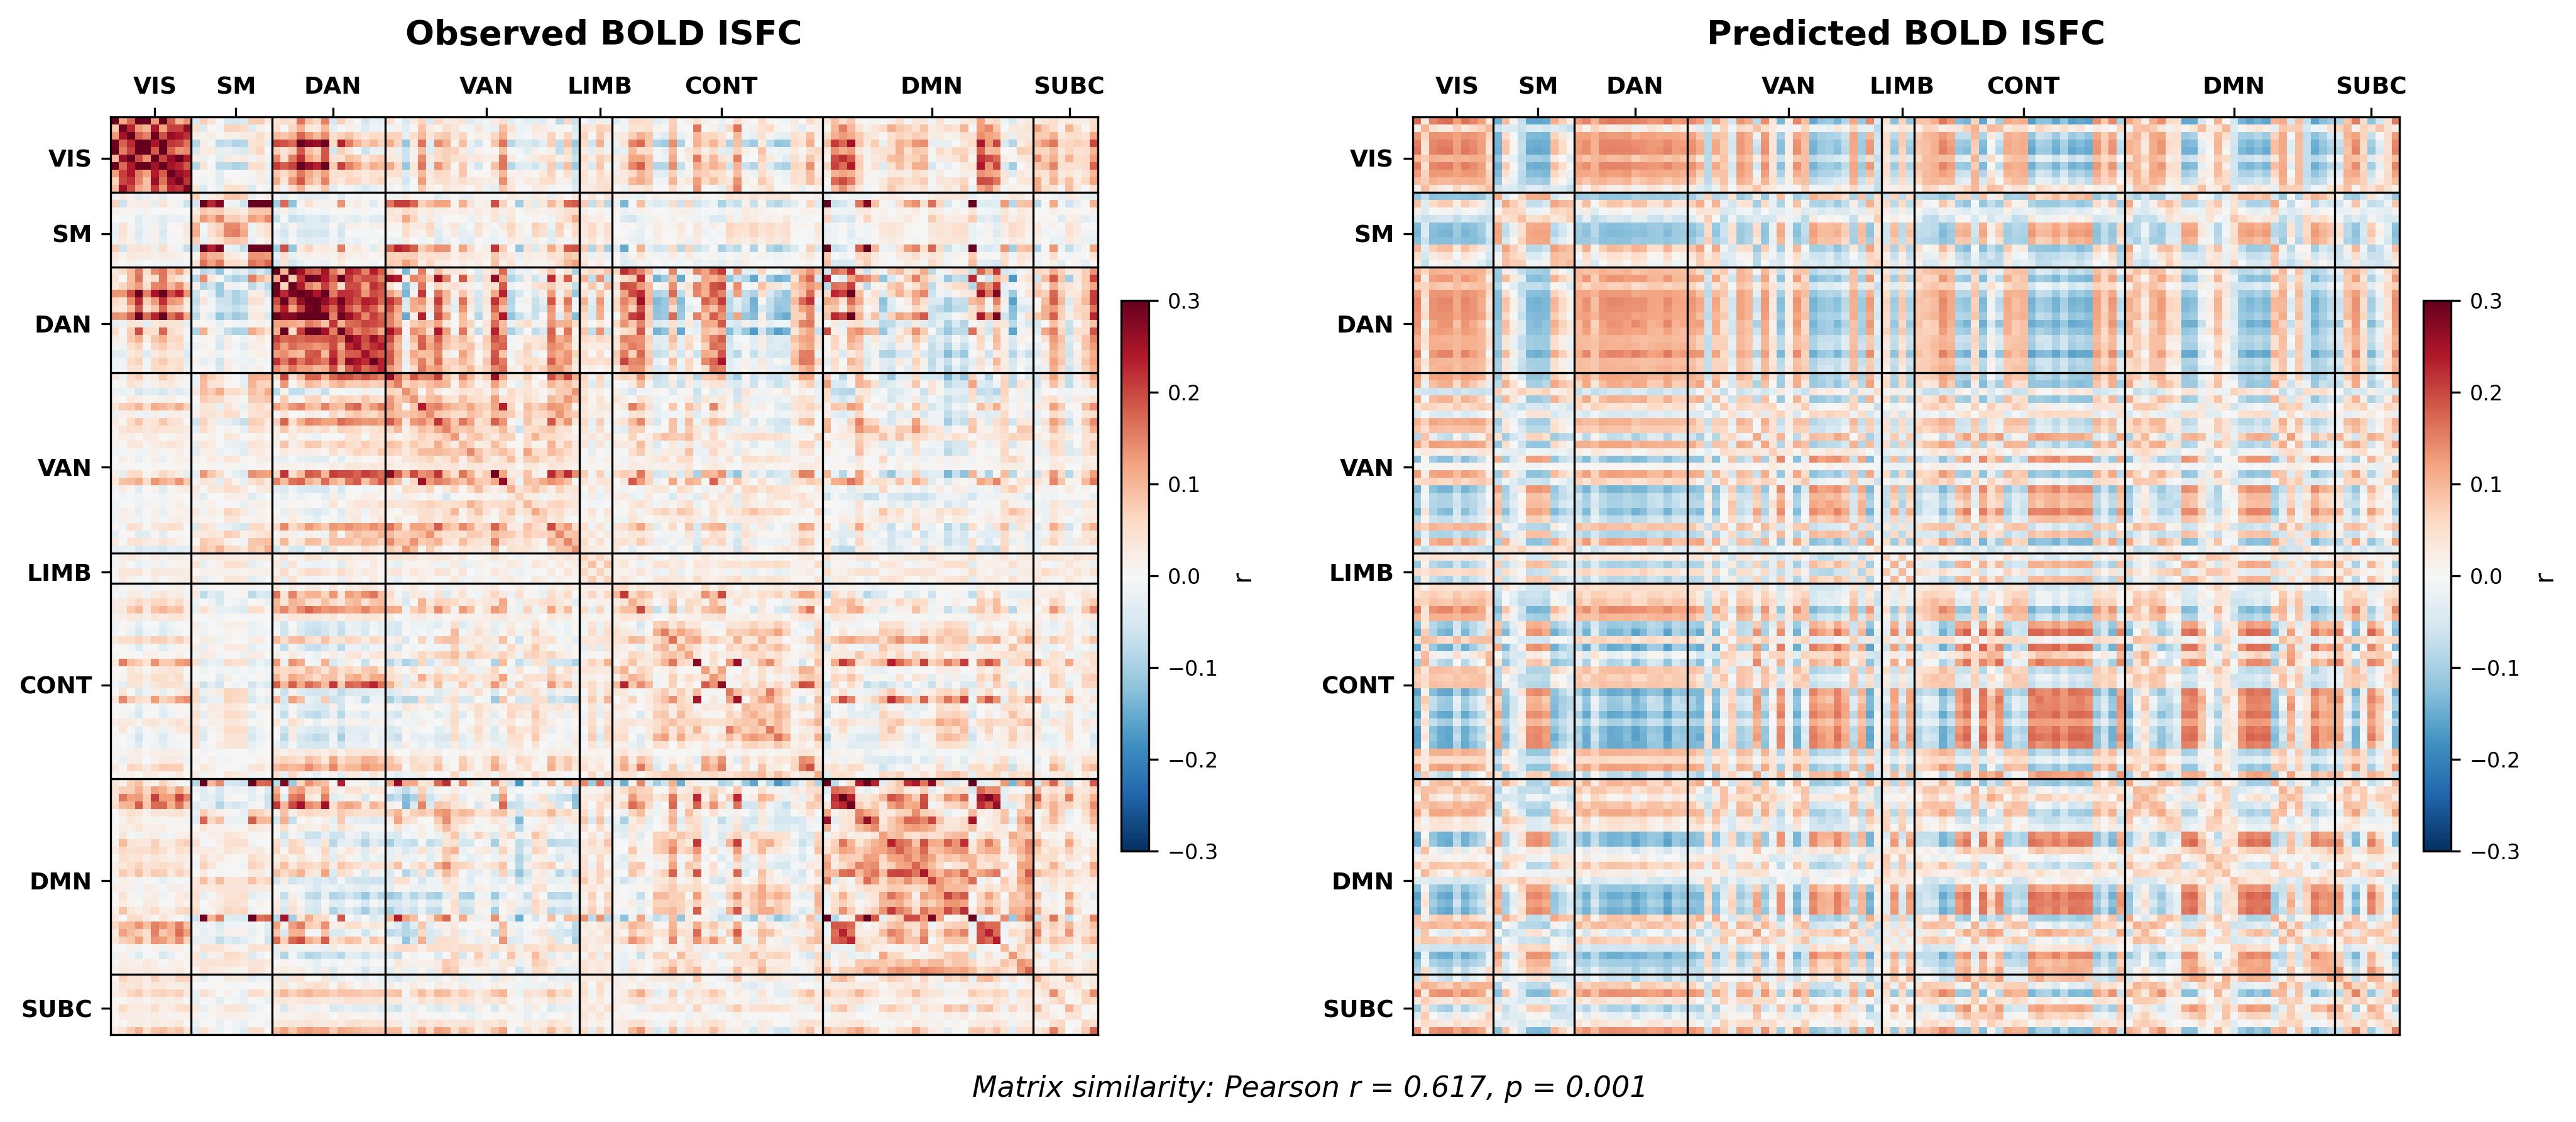
\includegraphics[width=0.55\textwidth, height=9cm, keepaspectratio]{../figures/fig4_isfc_heatmap.jpg}
    \end{figure}

    {\small \textbf{Figure 1.} Observed vs.\ predicted ISFC matrices. \textit{(continued in next column)}}

    \setcounter{figure}{1}

  \end{block}

\end{column}

\separatorcolumn

% ====================
% COLUMN 2: ISFC caption (continued), brain map, bar plot, replication, QR code
% ====================

\begin{column}{\colwidth}

  \begin{block}{Preliminary Results (continued)}

    {\small \textbf{Figure 1 (continued).} Observed (left) vs.\ predicted (right) inter-subject functional connectivity (ISFC) matrices. Each cell is the average correlation between one ROI's time series and the leave-one-out group mean. The Pearson correlation between the two matrices is $r = 0.552$ ($p = 0.001$, permutation test). The model preserves the antagonistic relationship between task-positive and default-mode networks.}

    \bigskip

    \heading{37 of 122 brain regions significantly predicted (FDR $q < 0.05$)}

    \begin{figure}
      \centering
      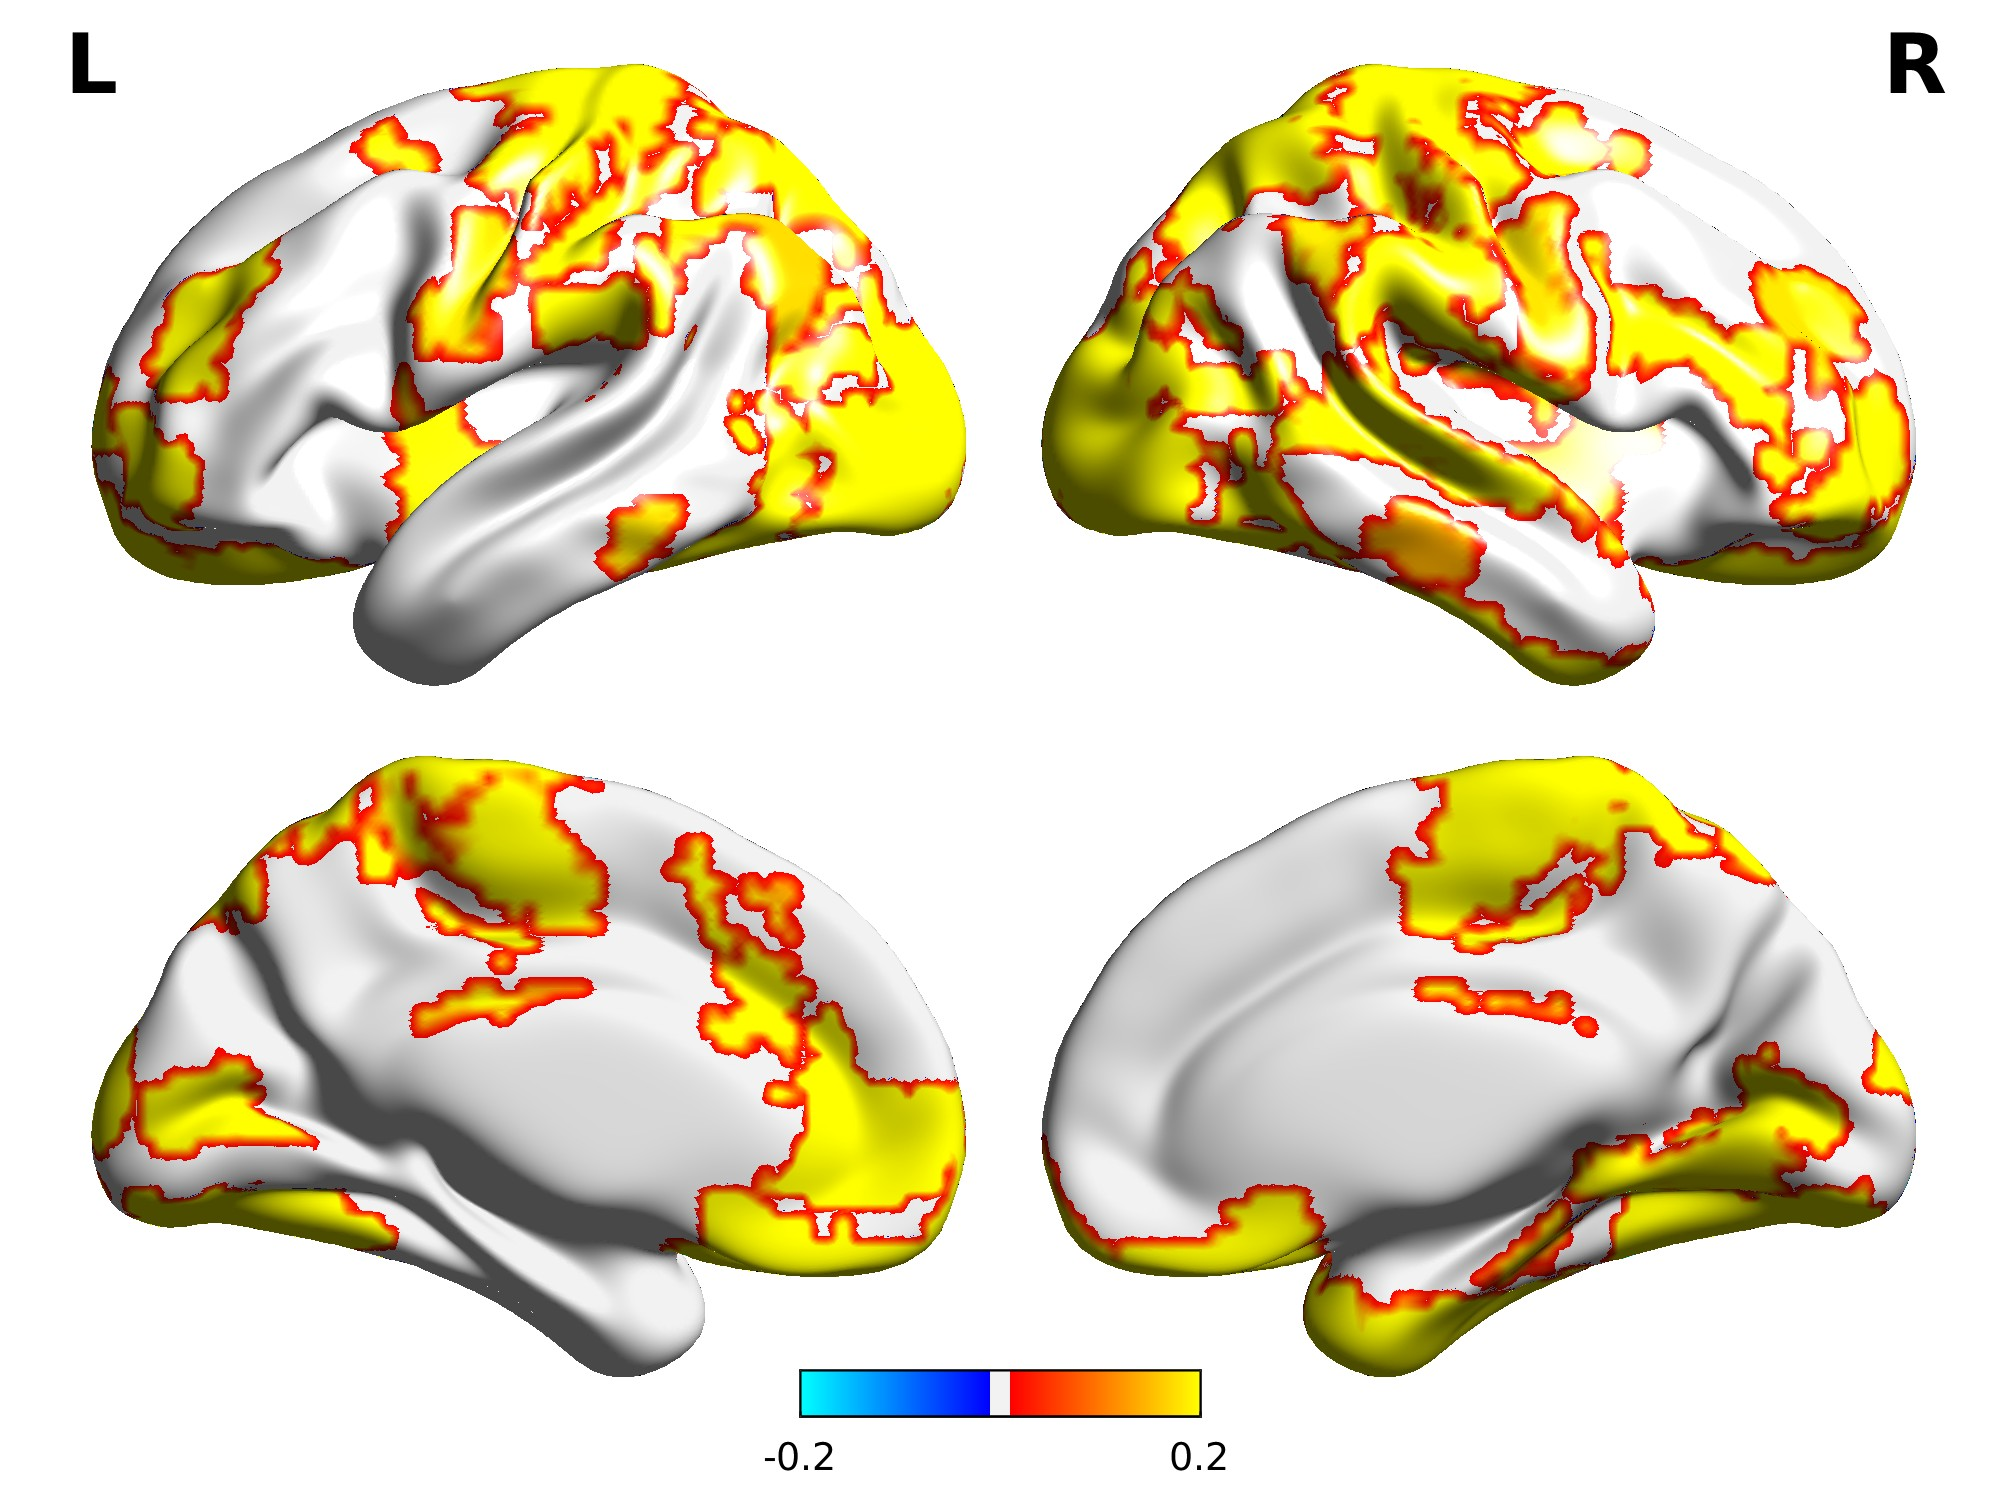
\includegraphics[width=0.75\textwidth]{../figures/fig3a_grp_grp_r_pmasked.jpg}
      \caption{Brain surface map of aPCR prediction accuracy (Pearson $r$ between predicted and observed fMRI). Warm colors = higher prediction accuracy; only FDR-significant ROIs ($q < 0.05$) highlighted. Significant prediction appears in visual, parietal, and prefrontal regions, including areas beyond direct fNIRS cap coverage, suggesting the model recovers network-level dynamics through temporal covariation.}
    \end{figure}

    \heading{Prediction distributed across attention-relevant networks}

    \begin{figure}
      \centering
      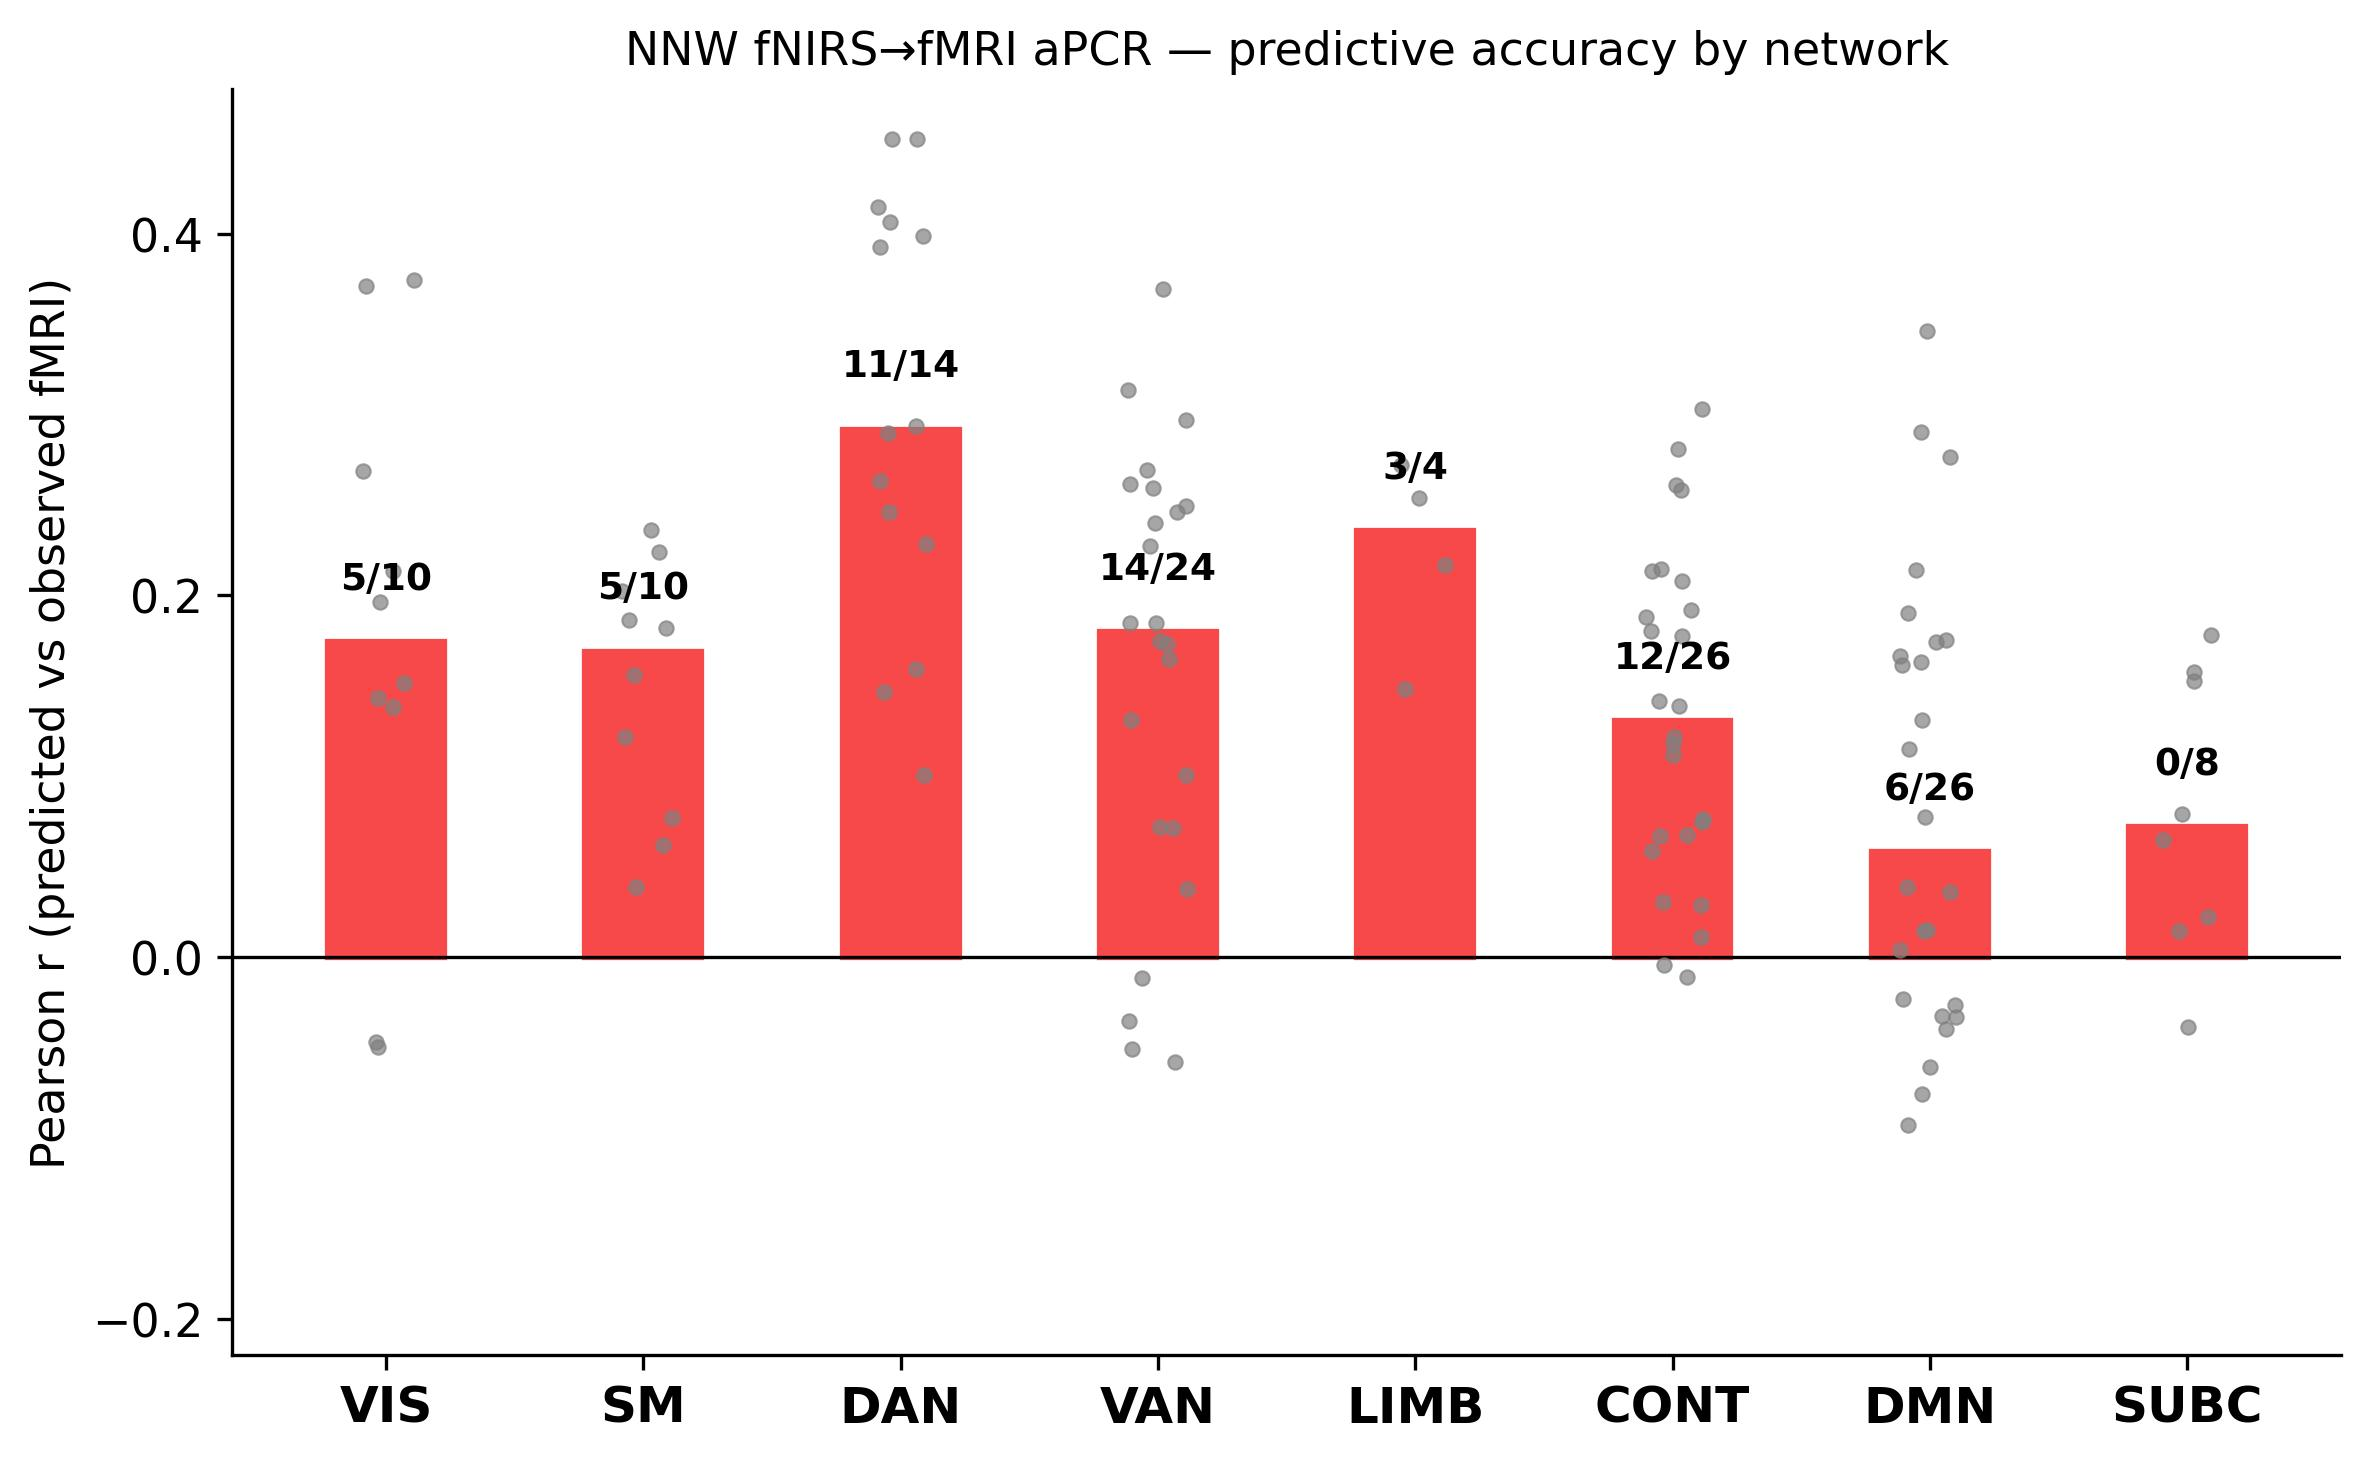
\includegraphics[width=0.75\textwidth]{../figures/fig3b_network_barplot.jpg}
      \caption{Prediction accuracy by functional network (Yeo 17-network atlas, collapsed to 8 systems). Bars = median Pearson $r$; dots = individual ROIs; fractions = significant/total per network. DAN (6/14), CONT (7/26), and DMN (7/26) account for 20 of 37 significant ROIs --- the three networks most implicated in attentional control.}
    \end{figure}

    \heading{Independent replication}

    Applying the identical pipeline to a separate fNIRS dataset (different participants, same film, same tasks) yielded 28 significantly predicted ROIs and ISFC $r = 0.297$ ($p = 0.001$), confirming the pipeline generalizes beyond a single dataset.

    \bigskip

    \begin{center}
      
\includegraphics[width=3cm]{figures/qr_references.png}\\[4pt]
      {\small Scan for full reference list}
    \end{center}

  \end{block}

\end{column}

\separatorcolumn

% ====================
% COLUMN 3: Expected Results, Key Takeaway, Limitations
% ====================

\begin{column}{\colwidth}

  \begin{block}{Expected Results: Individual Differences}

    \heading{Central hypothesis: DMN intrusion $\rightarrow$ attentional instability}

    During goal-directed tasks, the default mode network (DMN) is normally suppressed. When suppression fails, the DMN reactivates and disrupts processing, producing unusually slow and variable responses. Participants with higher predicted DMN activation during cognitive tasks should therefore show higher intraindividual reaction time variability (RTV), the standard behavioral marker of attentional lapses.

    \begin{figure}
      \centering
      \begin{minipage}{0.73\textwidth}
        \centering
        \textbf{\color{red}SIMULATED DATA}\\[2pt]
        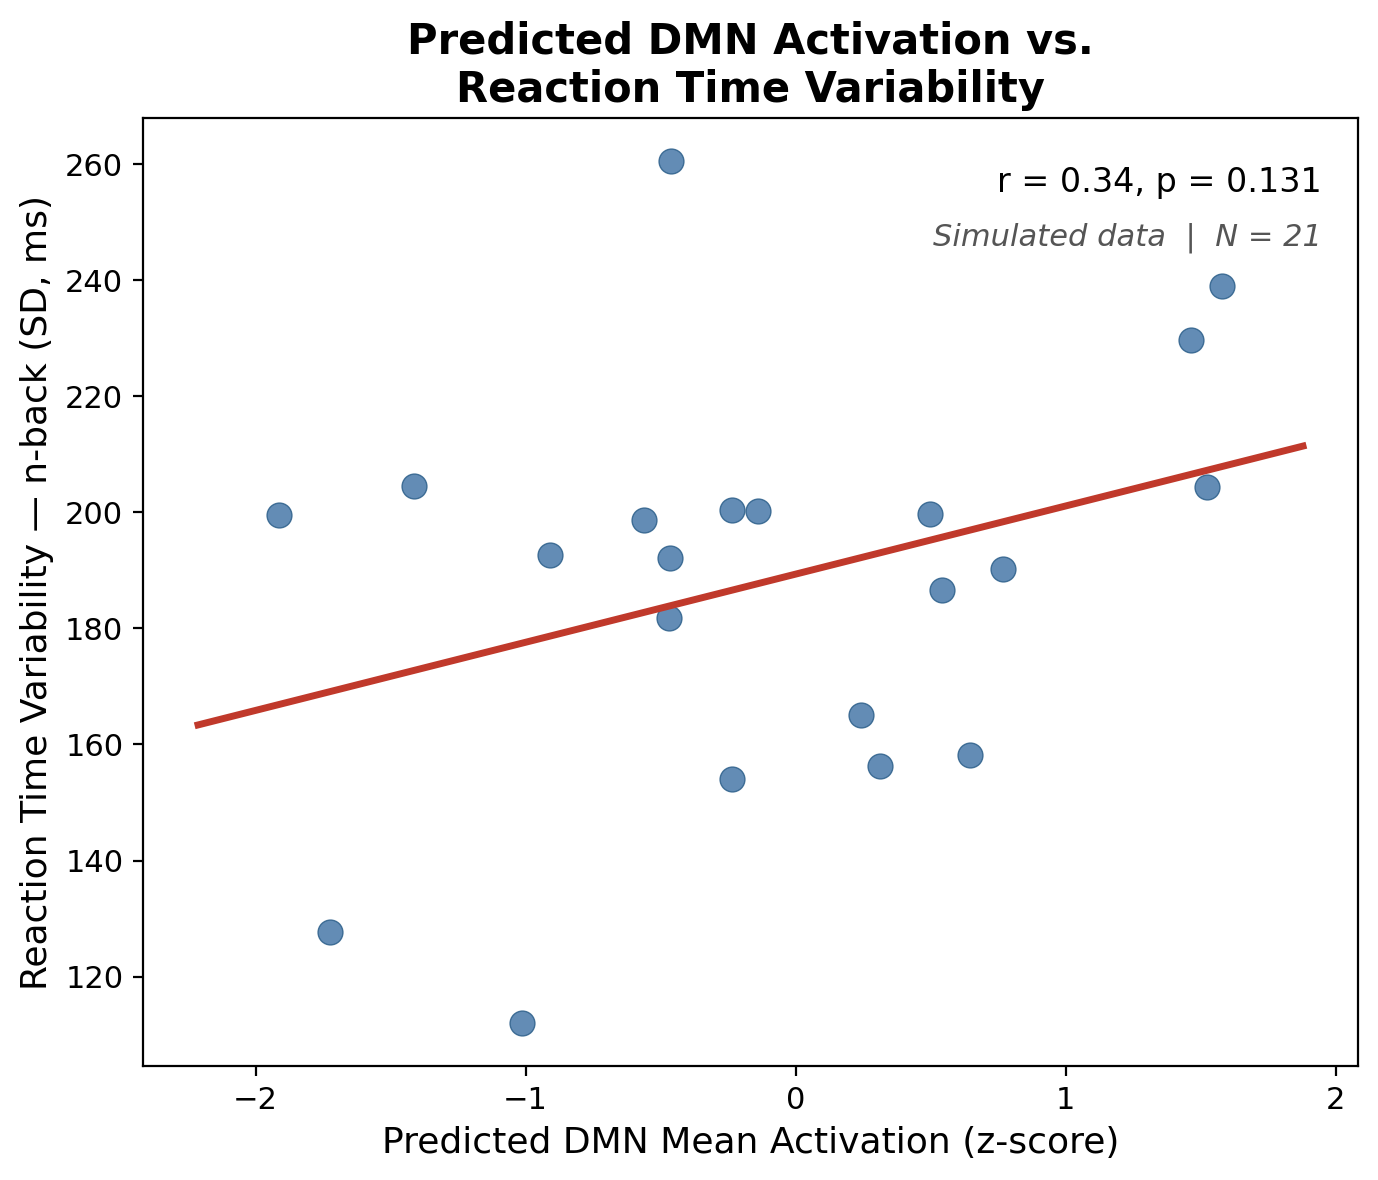
\includegraphics[width=\textwidth]{../figures/fig_mockup_dmn_rtv.png}
      \end{minipage}
      \caption{Mock data ($r = 0.34$, N\,=\,21) illustrating the predicted DMN--RTV relationship during n-back. \textbf{Not real data} --- included to show the expected pattern and effect size.}
    \end{figure}

    \heading{Planned analyses (specific tests)}

    \begin{enumerate}
      \item \textbf{Neural plausibility}: Within each subject's predicted fMRI, test whether mean DAN/CONT activation is higher in 2-back than 1-back, and DMN lower, via paired $t$-tests across subjects.
      \item \textbf{DMN--RTV correlation}: Correlate each subject's mean predicted DMN activation during n-back with their intraindividual SD of correct-trial RTs (iSD-RT). Expected $r \approx 0.40$.
      \item \textbf{Frontoparietal--accuracy}: Correlate predicted DAN/CONT activation with n-back accuracy and CPT d-prime. Mixed-effects models account for repeated measures.
      \item \textbf{Load sensitivity}: Compare prediction quality ($R^2$) for 1-back vs.\ 2-back to test whether the model tracks cognitive demand.
    \end{enumerate}

  \end{block}

  \begin{exampleblock}{Key Takeaway}

    \textbf{If} a 15-minute movie-watching fNIRS session can predict brain patterns that track individual differences in who pays attention, \textbf{then} whole-brain-equivalent neurocognitive assessment becomes feasible \textbf{without a scanner} --- in schools, clinics, and communities where MRI does not exist. The training-phase results establish the model captures real neural structure; the cognitive task analyses will determine how far that structure generalizes.

  \end{exampleblock}

  \begin{block}{Limitations}

    \begin{itemize}
      \item \textbf{Spatial coverage}: The fNIRS cap has no channels over medial prefrontal, visual, or subcortical areas. Predictions for those regions rely on learned covariation, not direct measurement.
      \item \textbf{Session ordering}: Movie-watching occurred after 2 hours of cognitive tasks; fatigue may have shifted the network profile toward VIS/DAN. Future collection will use movie-first ordering.
      \item \textbf{Sample size}: N\,=\,21 is underpowered for effects below $r \approx 0.40$. Recruiting toward N\,=\,40; effect sizes and CIs will be reported regardless.
      \item \textbf{No task fMRI ground truth}: Cross-task validation is indirect (ISFC, behavior, literature). HCP n-back (N\,=\,1{,}200) available as external benchmark if needed.
    \end{itemize}

  \end{block}

\end{column}

\separatorcolumn
\end{columns}
\end{frame}

\end{document}